\section{Evaluation Protocol}

\label{sec:protocol}
Building on the construction in \S~3, this section specifies how each \textsc{TIDE-Bench} sample is turned into an evaluation run for the experiments below.


\subsection{Interaction Setup}
\label{subsec:interaction}

Each \textsc{TIDE-Bench} sample defines a dialogue task where an agent interacts with a user simulator (\S~\ref{subsec:simulator}) over a database $\mathcal{D}$ with schema $\mathcal{S}$. The dialogue begins with the user's initial question $u_1$ and proceeds in alternating turns $(u_1, a_1, u_2, a_2, \ldots)$. Each agent turn $a_i$ is either a clarification request or candidate SQL query against $\mathcal{D}$; the simulator returns $u_{i+1}$. For Drift-only and Joint samples, the harness injects the pre-annotated drift turn verbatim after the agent's first SQL query, ensuring deterministic drift content across evaluation runs.

\namedpara{\(\boldsymbol{f}\)-protocol and \(\boldsymbol{p}\)-protocol.} Each sample is evaluated under two protocols. The \textbf{\(\boldsymbol{f}\)-protocol} (\emph{full}) starts from $u_1$, requiring the agent to elicit and resolve both clarification layers for Chain-only and Joint samples. The \textbf{\(\boldsymbol{p}\)-protocol} (L1-\emph{primed}) pre-populates the history with a synthetic three-turn L1 resolution: the initial question, annotated L1 clarification, and canonical L1 answer. It marks the simulator's L1 state as resolved before the first live turn. The $p$-protocol isolates L2, testing whether agents miss it once L1 is no longer a confound. Full harness parameter settings appear in Appendix~\ref{app:evaluation-setup}.

\subsection{User Simulator}
\label{subsec:simulator}

The simulator follows the two-stage function-driven design of recent advance~\cite{huo2026interact}, with three minor adaptations for \textsc{TIDE-Bench}'s two-layer chain structure (Appendix~\ref{app:user-sim}). The router decisions $\rho_t$ used by  the metrics below are produced at each user turn responding to an agent clarification. We validate the simulator on USERSIM-GUARD and on agent--simulator traces independently labeled by five SQL experts (Fleiss' $\kappa = 0.802$); full configuration provided in Appendix~\ref{app:user-sim}.



\subsection{Metrics}
\label{subsec:metrics}

Seven metrics span four behavioral facets: execution accuracy, clarification behavior, chain-layer identification and drift handling. All are computed as proportions over a sample set $\mathcal{S}$ of a given type.

\namedpara{Notation.}
Let $\tau$ denote a dialogue trajectory containing $n_\tau \in \{1, 2\}$ SQL queries $y_1, \ldots, y_{n_\tau}$ paired with $y_1^*, \ldots, y_{n_\tau}^*$. Chain-only samples have $n_\tau = 1$, while Drift-only and Joint samples have $n_\tau = 2$, with $y_1 = y_{\mathrm{pre}}$ and $y_2 = y_{\mathrm{post}}$. Let
$\mathrm{EX}(y, y^*) \in \{0, 1\}$ denote execution match, i.e., equivalent result sets modulo row order; $\rho_t \in \{\mathrm{L1}, \mathrm{L2}, \mathrm{Other}\}$ denote the router decision (\S~\ref{subsec:simulator}) for the agent's clarification at turn $t$; and $S(y)$ denote the commitment set of $y$ (\S~\ref{subsec:drift}). Define $\mathrm{Rec}(\tau) := \bigl[ S(y_{\mathrm{pre}}) \nsubseteq S(y_{\mathrm{post}}) \bigr]$ as the non-monotonicity condition used for drift recognition.

\begin{table*}[t]
\centering
\small
\setlength{\tabcolsep}{3pt}
\renewcommand{\arraystretch}{1.52}

\begin{tabular*}{\linewidth}{
@{}
c@{\hspace{4pt}}
l@{\hspace{6pt}}
c@{\extracolsep{\fill}}
c c c c c c c c
@{}
}

\toprule
\multirow{2}{*}{\textbf{\#}}
& \multicolumn{1}{c@{\hspace{6pt}}}
  {\multirow{2}{*}{\textbf{Model}}}
& \multirow{2}{*}{\textbf{Chain-only}}
& \multicolumn{4}{c}{\textbf{Drift-only}}
& \multicolumn{4}{c}{\textbf{Joint}} \\
\cmidrule(lr){4-7}
\cmidrule(lr){8-11}

& &
& \textbf{Value}
& \textbf{Constraint}
& \textbf{Projection}
& \textbf{All}
& \textbf{Value}
& \textbf{Constraint}
& \textbf{Projection}
& \textbf{All} \\

\midrule
1  & Claude-Sonnet-4.6 & \textbf{35.9} & \textbf{47.7} & \textbf{44.2} & 43.4 & \textbf{45.1} & \textbf{31.2} & 20.2 & \textbf{31.4} & \textbf{27.8} \\
2  & Qwen2.5-72B       & 32.4 & 44.3 & 41.1 & \underline{44.0} & \underline{43.2} & \underline{30.1} & \underline{21.5} & 28.6 & \underline{26.8} \\
3  & o4-mini           & \underline{32.9} & 42.6 & 41.1 & 40.0 & 41.2 & \textbf{31.2} & \underline{21.5} & 27.4 & \underline{26.8} \\
4  & GPT-4o            & 30.9 & \underline{46.0} & 38.7 & \textbf{44.6} & \underline{43.2} & 27.8 & \textbf{22.1} & \underline{29.7} & 26.7 \\
5  & GPT-5.4           & 32.5 & 43.2 & 36.8 & 42.3 & 40.9 & 27.8 & 20.9 & \underline{29.7} & 26.3 \\
6  & Llama-3.3-70B     & 32.7 & 40.3 & 39.3 & 38.9 & 39.5 & 29.5 & \textbf{22.1} & 26.9 & 26.3 \\
7  & o3-mini           & 32.6 & 40.9 & 37.4 & 38.9 & 39.1 & 29.5 & 18.4 & 28.6 & 25.7 \\
8  & Gemini-2.5-Flash  & 31.6 & 39.2 & 42.9 & 33.1 & 38.3 & 27.3 & 20.2 & 27.4 & 25.1 \\
9  & Grok-4.1-Fast     & 30.4 & 41.5 & 36.2 & 41.7 & 39.9 & 29.0 & 18.4 & 25.1 & 24.3 \\
10 & Qwen-Max          & 30.5 & 40.3 & \underline{43.6} & 40.6 & 41.4 & 28.4 & 20.9 & 21.7 & 23.7 \\
11 & DeepSeek-V4-Flash & 27.3 & 40.9 & 39.9 & 39.4 & 40.1 & 21.6 & 17.8 & 26.9 & 22.2 \\
12 & Grok-4-Fast       & 25.9 & 36.9 & 33.7 & 38.9 & 36.6 & 19.9 & 14.7 & 22.9 & 19.3 \\
\bottomrule

\end{tabular*}

\vspace{-1mm}
\caption{DEA (\%) under the paired factorial design. The best and second-best results per column are in bold and underlined, respectively. Chain-only reports strict execution accuracy; Drift-only and Joint report end-to-end accuracy broken down by drift subtype; All denotes aggregate performance, and higher metric values are better.}
\label{tab:dea}
\vspace{-1mm}
\end{table*}
\begin{figure*}[!t]
  \centering
  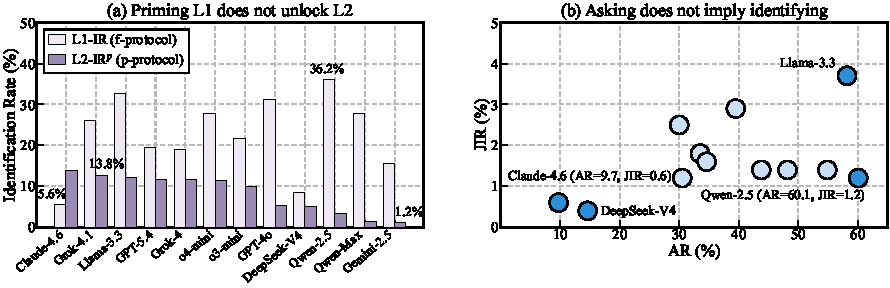
\includegraphics[width=\textwidth]{figure/chain_identification.pdf}
  \vspace{-7mm}
  \caption{Chain-layer identification on Chain-only samples. (a) L1-IR ($f$-protocol) vs.\ L2-IR$^p$ ($p$-protocol) per model: even with L1 pre-resolved, L2 identification stays low. (b) JIR against ask rate: identification remains low regardless of how much the agent asks. Model names are abbreviated; full names appear in Table~\ref{tab:dea} for reference.}
  \label{fig:chain}
  \vspace{-5mm}
\end{figure*}

\namedpara{Metric definitions.} The seven metrics are defined in Table~\ref{tab:metrics}. \textbf{DEA} requires every SQL query in a trajectory to pass execution match. \textbf{AR} measures whether the agent asks, regardless of layer, providing a baseline clarification rate. \textbf{L1-IR}, \textbf{L2-IR$^{p}$}, and \textbf{JIR} measure whether the agent surfaces clarification requests routed to the corresponding layer within a trajectory, with L2-IR$^{p}$ evaluated under the $p$-protocol to isolate L2 from L1 confounds. \textbf{DRR} captures whether the agent's commitment sets exhibit the required non-monotonic change after the drift utterance, and \textbf{DRA} additionally requires the resulting post-drift SQL to be executionally correct. 

